% Krino -- long-list readout strategies at K = 150
% Build: make build   (pdflatex twice in oaklight/texlive:science-cn)
\documentclass[tikz,border=10pt]{standalone}
\usepackage{amsmath}
\usepackage{amssymb}
\usetikzlibrary{arrows.meta,positioning,calc,decorations.pathreplacing,shapes.geometric}

% ---------------------------------------------------------------- palette
% Same palette and type as research/figures/architecture/architecture.tex.
\definecolor{frozenfill}{HTML}{F3F4F6}
\definecolor{frozendraw}{HTML}{6B7280}
\definecolor{trainfill}{HTML}{EFF6FF}
\definecolor{trainraw}{HTML}{2563EB}
\definecolor{fusefill}{HTML}{F5F3FF}
\definecolor{fusedraw}{HTML}{7C3AED}
\definecolor{lossfill}{HTML}{FFFBEB}
\definecolor{lossdraw}{HTML}{D97706}
\definecolor{notefill}{HTML}{FAFAF9}

\tikzset{
  box/.style={rounded corners=3pt, draw, line width=0.6pt, align=center,
              inner sep=5pt, font=\sffamily\small},
  plain/.style={box, draw=black!35, fill=white},
  note/.style={rounded corners=3pt, draw=black!30, line width=0.5pt,
               fill=notefill, align=flush left, inner sep=5pt,
               font=\sffamily\scriptsize},
  sched/.style={rounded corners=2.5pt, draw, line width=0.7pt, align=center,
                inner sep=4pt, font=\sffamily\scriptsize},
  schemea/.style={sched, fill=lossfill, draw=lossdraw},
  schemeB/.style={sched, fill=trainfill, draw=trainraw},
  schemeC/.style={sched, fill=fusefill, draw=fusedraw},
  refbox/.style={sched, fill=frozenfill, draw=frozendraw, dashed},
  arrow/.style={-{Stealth[length=2.2mm,width=1.6mm]}, line width=0.6pt,
                draw=black!70},
  alabel/.style={font=\sffamily\scriptsize, text=black!65, align=center},
  ptitle/.style={font=\sffamily\large\bfseries, text=black!85},
  psub/.style={font=\sffamily\scriptsize, text=black!60, align=flush left},
  tick/.style={font=\sffamily\scriptsize, text=black!60},
  mka/.style={rectangle, fill=lossdraw, draw=lossdraw, inner sep=1.2pt,
              minimum size=3.0pt},
  mkB/.style={circle, fill=trainraw, draw=trainraw, inner sep=1.2pt,
              minimum size=3.0pt},
  mkC/.style={diamond, fill=fusedraw, draw=fusedraw, inner sep=1.2pt,
              minimum size=3.4pt},
  mkJ/.style={rectangle, fill=black!55, draw=black!55, inner sep=1.2pt,
              minimum size=3.0pt},
  mkS/.style={circle, fill=frozendraw, draw=frozendraw, inner sep=1.1pt,
              minimum size=2.8pt},
}

\begin{document}
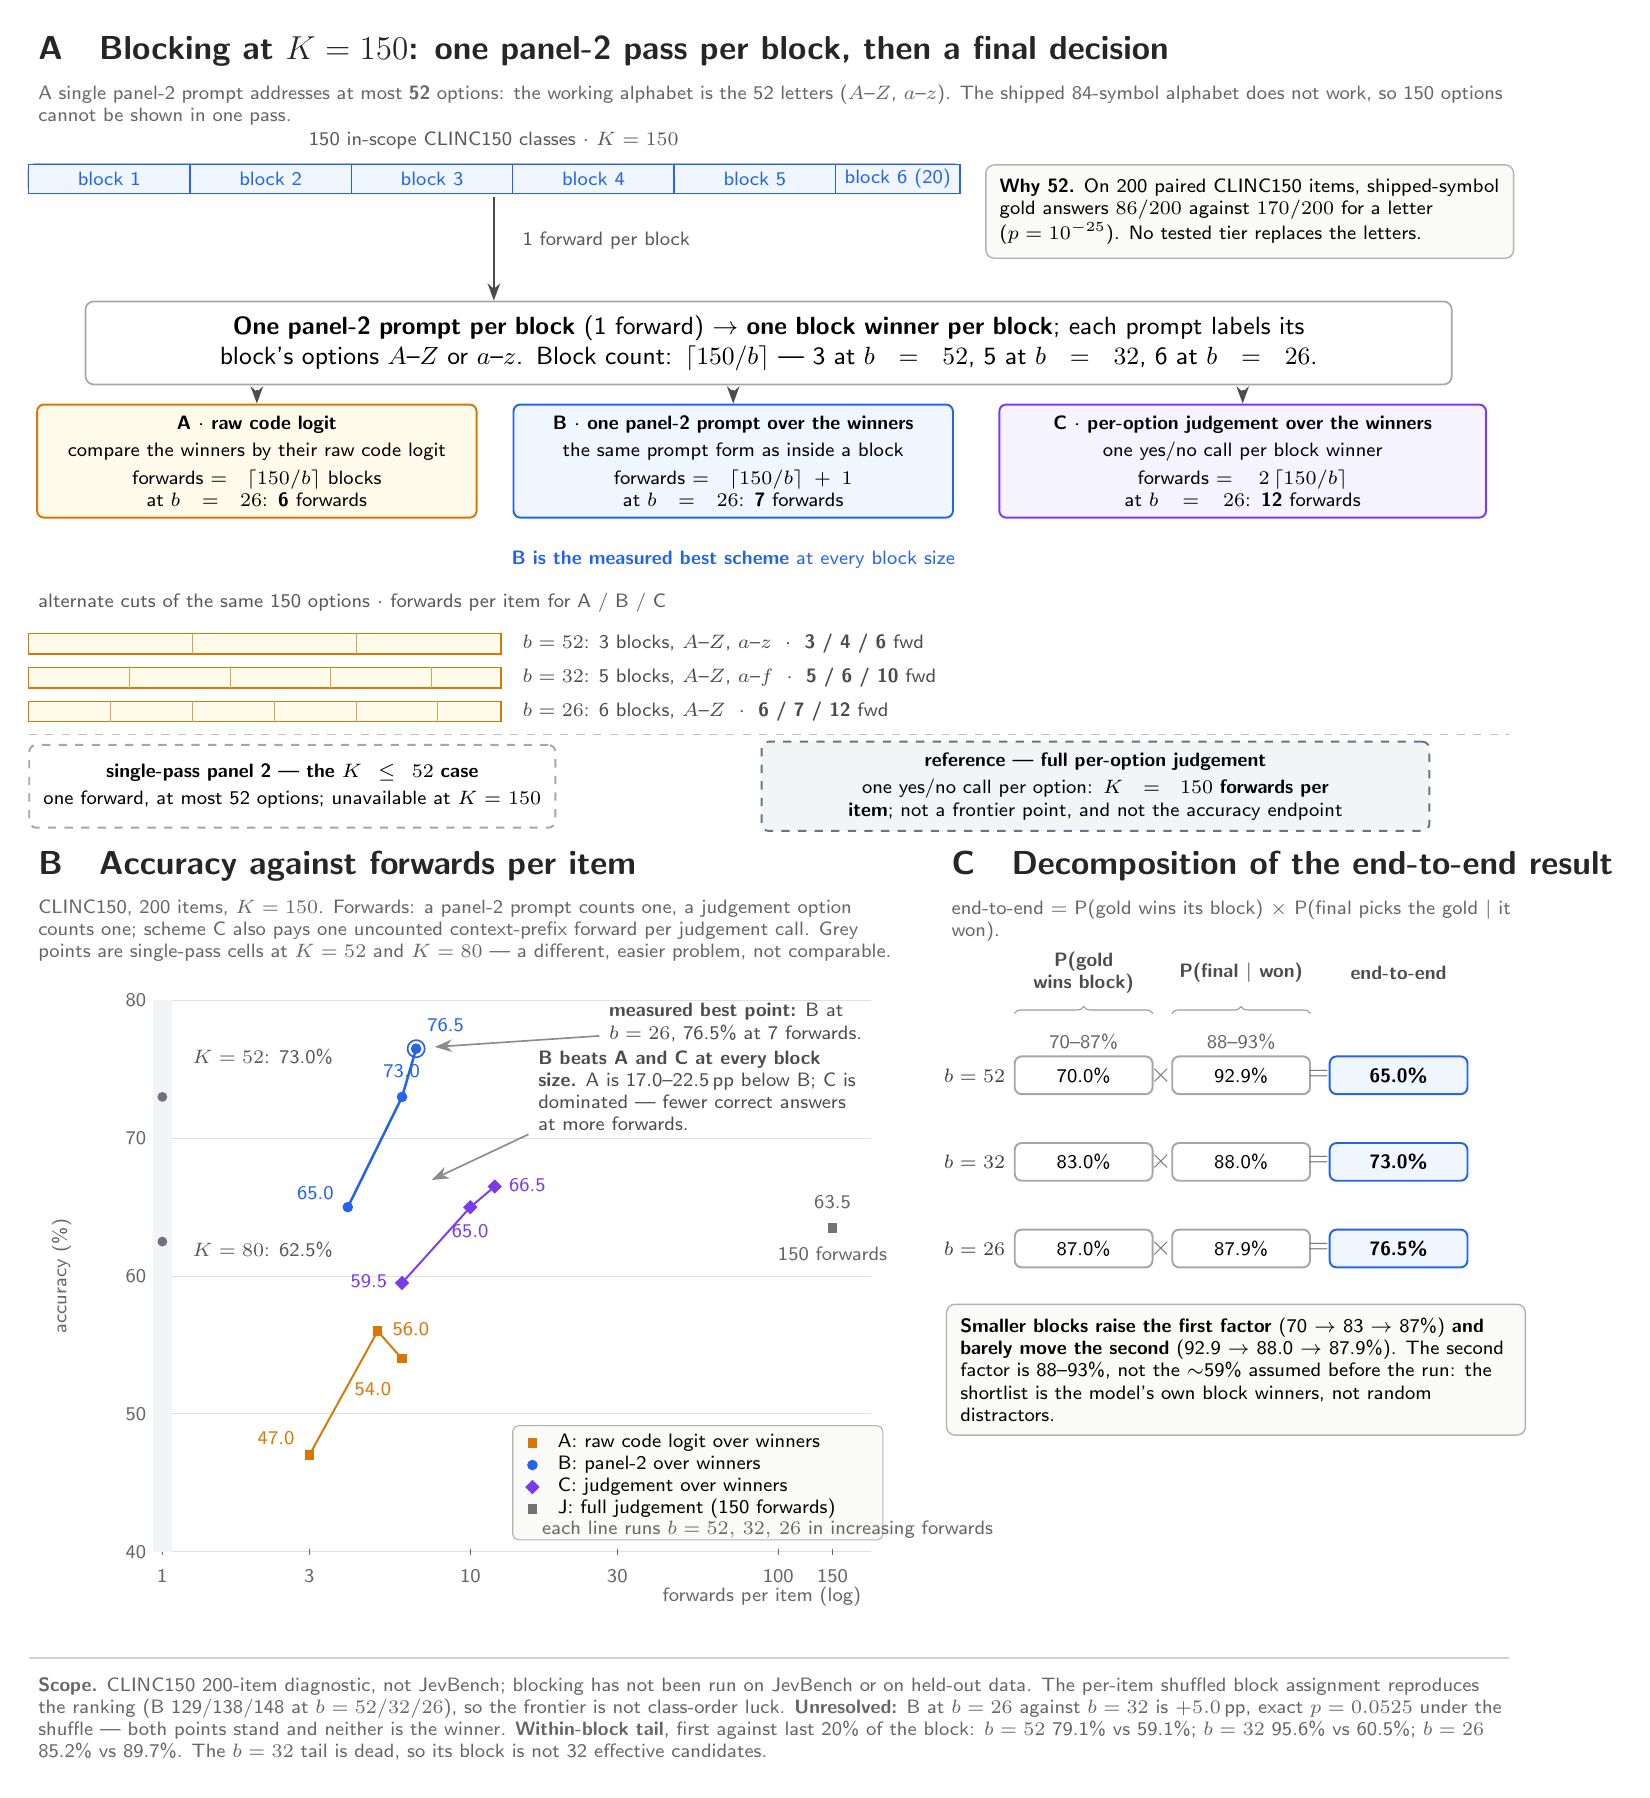
\begin{tikzpicture}[font=\sffamily]

% =====================================================================
% PANEL A -- schematic at K = 150
% =====================================================================
\node[ptitle, anchor=west] at (0.20,19.95)
  {A\quad Blocking at $K=150$: one panel-2 pass per block, then a final decision};
\node[psub, anchor=north west, text width=18.6cm] at (0.20,19.65)
  {A single panel-2 prompt addresses at most \textbf{52} options: the working alphabet is the 52 letters
   ($A$--$Z$, $a$--$z$). The shipped 84-symbol alphabet does not work, so 150 options cannot be shown in one pass.};

% --- input strip: 150 options cut into 6 blocks of 26 (last 20)
\node[alabel, anchor=south] at (6.11,18.58)
  {150 in-scope CLINC150 classes $\cdot$ $K=150$};
\draw[fill=white, draw=black!45, line width=0.6pt, rounded corners=2pt]
  (0.20,18.15) rectangle (12.03,18.52);
\foreach \i/\xa/\xb in {1/0.20/2.25, 2/2.25/4.30, 3/4.30/6.35,
                        4/6.35/8.40, 5/8.40/10.45} {
  \draw[fill=trainfill, draw=trainraw, line width=0.5pt] (\xa,18.15) rectangle (\xb,18.52);
  \node[font=\sffamily\scriptsize, text=trainraw] at ({(\xa+\xb)/2},18.335) {block \i};
}
\draw[fill=trainfill, draw=trainraw, line width=0.5pt] (10.45,18.15) rectangle (12.03,18.52);
\node[font=\sffamily\scriptsize, text=trainraw] at (11.24,18.335) {block 6 (20)};

% --- constraint note beside the strip
\node[note, anchor=north west, text width=6.35cm] at (12.35,18.52)
  {\textbf{Why 52.} On 200 paired CLINC150 items, shipped-symbol gold answers
   $86/200$ against $170/200$ for a letter ($p=10^{-25}$).
   No tested tier replaces the letters.};

% --- block winners
\node[plain, text width=17.0cm] (winners) at (9.60,16.25)
  {\textbf{One panel-2 prompt per block} (1 forward) $\to$ \textbf{one block winner per block};
   each prompt labels its block's options $A$--$Z$ or $a$--$z$. Block count: $\lceil 150/b\rceil$ ---
   3 at $b=52$, 5 at $b=32$, 6 at $b=26$.};
\draw[arrow] (6.11,18.10) -- (winners.north -| 6.11,0);
\node[alabel, anchor=west] at (6.35,17.55) {1 forward per block};

% --- three final-decision variants
\node[schemea, text width=5.3cm, minimum height=1.40cm] (sa) at (3.10,14.75)
  {\textbf{A $\cdot$ raw code logit}\\[2pt]
   compare the winners by their raw code logit\\[2pt]
   forwards $=\lceil 150/b\rceil$ blocks\\
   at $b=26$: \textbf{6} forwards};
\node[schemeB, text width=5.3cm, minimum height=1.40cm] (sb) at (9.15,14.75)
  {\textbf{B $\cdot$ one panel-2 prompt over the winners}\\[2pt]
   the same prompt form as inside a block\\[2pt]
   forwards $=\lceil 150/b\rceil+1$\\
   at $b=26$: \textbf{7} forwards};
\node[schemeC, text width=5.9cm, minimum height=1.40cm] (sc) at (15.62,14.75)
  {\textbf{C $\cdot$ per-option judgement over the winners}\\[2pt]
   one yes/no call per block winner\\[2pt]
   forwards $=2\,\lceil 150/b\rceil$\\
   at $b=26$: \textbf{12} forwards};
\draw[arrow] (3.10,15.65) -- (sa.north);
\draw[arrow] (9.15,15.65) -- (sb.north);
\draw[arrow] (15.62,15.65) -- (sc.north);
\node[font=\sffamily\scriptsize, text=trainraw, align=center] at (9.15,13.50)
  {\textbf{B is the measured best scheme} at every block size};

% --- alternate cuts of the same list
\node[alabel, anchor=west] at (0.20,12.95)
  {alternate cuts of the same 150 options $\cdot$ forwards per item for A / B / C};
\foreach \y in {12.30, 11.87, 11.44} {
  \draw[fill=lossfill, draw=lossdraw, line width=0.5pt] (0.20,\y) rectangle (6.20,\y+0.26);
}
% b = 52: 2 full blocks, last 46
\draw[lossdraw!70, line width=0.35pt] (2.28,12.30) -- (2.28,12.56);
\draw[lossdraw!70, line width=0.35pt] (4.36,12.30) -- (4.36,12.56);
\node[anchor=west, font=\sffamily\scriptsize, text=black!70] at (6.35,12.43)
  {$b=52$: 3 blocks, $A$--$Z$, $a$--$z$ $\;\cdot\;$ \textbf{3 / 4 / 6} fwd};
% b = 32: 4 full blocks, last 22
\foreach \x in {1.48, 2.76, 4.04, 5.32}
  \draw[lossdraw!70, line width=0.35pt] (\x,11.87) -- (\x,12.13);
\node[anchor=west, font=\sffamily\scriptsize, text=black!70] at (6.35,12.00)
  {$b=32$: 5 blocks, $A$--$Z$, $a$--$f$ $\;\cdot\;$ \textbf{5 / 6 / 10} fwd};
% b = 26: 5 full blocks, last 20
\foreach \x in {1.24, 2.28, 3.32, 4.36, 5.40}
  \draw[lossdraw!70, line width=0.35pt] (\x,11.44) -- (\x,11.70);
\node[anchor=west, font=\sffamily\scriptsize, text=black!70] at (6.35,11.57)
  {$b=26$: 6 blocks, $A$--$Z$ $\;\cdot\;$ \textbf{6 / 7 / 12} fwd};

% --- reference row, clearly separated
\draw[draw=black!25, dashed, line width=0.5pt] (0.20,11.28) -- (19.00,11.28);
\node[refbox, text width=6.4cm, minimum height=1.05cm, draw=black!35, fill=white]
  (refsingle) at (3.55,10.62)
  {\textbf{single-pass panel 2 --- the $K\le 52$ case}\\[2pt]
   one forward, at most 52 options; unavailable at $K=150$};
\node[refbox, text width=8.2cm, minimum height=1.05cm] (refjudge) at (13.75,10.62)
  {\textbf{reference --- full per-option judgement}\\[2pt]
   one yes/no call per option: \textbf{$K=150$ forwards per item};
   not a frontier point, and not the accuracy endpoint};

% =====================================================================
% PANEL B -- accuracy against forwards
% =====================================================================
\node[ptitle, anchor=west] at (0.20,9.60) {B\quad Accuracy against forwards per item};
\node[psub, anchor=north west, text width=10.9cm] at (0.20,9.30)
  {CLINC150, 200 items, $K=150$. Forwards: a panel-2 prompt counts one, a judgement option counts one;
   scheme C also pays one uncounted context-prefix forward per judgement call.
   Grey points are single-pass cells at $K=52$ and $K=80$ --- a different, easier problem, not comparable.};

% axes
\draw[black!60, line width=0.6pt] (1.90,0.90) -- (1.90,7.90);
\draw[black!60, line width=0.6pt] (1.90,0.90) -- (10.90,0.90);
\foreach \acc in {40,50,60,70,80} {
  \pgfmathsetmacro{\yy}{0.90 + 7.00*(\acc-40)/40}
  \draw[black!12, line width=0.4pt] (1.90,\yy) -- (10.90,\yy);
  \draw[black!60, line width=0.4pt] (1.86,\yy) -- (1.94,\yy);
  \node[tick, anchor=east] at (1.82,\yy) {\acc};
}
\foreach \f in {1,3,10,30,100,150} {
  \pgfmathsetmacro{\xx}{1.90 + 9.00*ln(\f)/ln(200)}
  \draw[black!60, line width=0.4pt] (\xx,0.86) -- (\xx,0.94);
  \node[tick, anchor=north] at (\xx,0.80) {\f};
}
\node[font=\sffamily\scriptsize, text=black!60, rotate=90] at (0.62,4.40) {accuracy (\%)};
\node[tick, anchor=north east] at (10.90,0.58) {forwards per item (log)};

% grey band: the single-pass cells, a different problem
\fill[frozenfill] (1.78,0.90) rectangle (2.02,7.90);
\node[mkS] at (1.90,{0.90+7.00*33.0/40}) {};
\node[mkS] at (1.90,{0.90+7.00*22.5/40}) {};
\node[font=\sffamily\scriptsize, text=black!65, anchor=west] at (2.16,7.18) {$K=52$: 73.0\%};
\node[font=\sffamily\scriptsize, text=black!65, anchor=west] at (2.16,4.74) {$K=80$: 62.5\%};

% scheme A: 47.0 / 56.0 / 54.0
\draw[lossdraw, line width=0.7pt]
  (3.766,{0.90+7.00*7.0/40}) -- (4.634,{0.90+7.00*16.0/40}) -- (4.944,{0.90+7.00*14.0/40});
\node[mka] (a1) at (3.766,{0.90+7.00*7.0/40}) {};
\node[mka] (a2) at (4.634,{0.90+7.00*16.0/40}) {};
\node[mka] (a3) at (4.944,{0.90+7.00*14.0/40}) {};

% scheme B: 65.0 / 73.0 / 76.5
\draw[trainraw, line width=0.9pt]
  (4.255,{0.90+7.00*25.0/40}) -- (4.944,{0.90+7.00*33.0/40}) -- (5.123,{0.90+7.00*36.5/40});
\node[mkB] (b1) at (4.255,{0.90+7.00*25.0/40}) {};
\node[mkB] (b2) at (4.944,{0.90+7.00*33.0/40}) {};
\node[mkB] (b3) at (5.123,{0.90+7.00*36.5/40}) {};
\draw[trainraw, line width=0.6pt] (b3) circle (3.1pt);

% scheme C: 59.5 / 65.0 / 66.5
\draw[fusedraw, line width=0.7pt]
  (4.944,{0.90+7.00*19.5/40}) -- (5.811,{0.90+7.00*25.0/40}) -- (6.121,{0.90+7.00*26.5/40});
\node[mkC] (c1) at (4.944,{0.90+7.00*19.5/40}) {};
\node[mkC] (c2) at (5.811,{0.90+7.00*25.0/40}) {};
\node[mkC] (c3) at (6.121,{0.90+7.00*26.5/40}) {};

% full judgement
\node[mkJ] (j1) at (10.411,{0.90+7.00*23.5/40}) {};

% accuracy labels
\node[font=\sffamily\scriptsize, text=lossdraw, anchor=east]
  at (3.70,{0.90+7.00*7.0/40+0.22}) {47.0};
\node[font=\sffamily\scriptsize, text=lossdraw, anchor=west]
  at (4.70,{0.90+7.00*16.0/40+0.02}) {56.0};
\node[font=\sffamily\scriptsize, text=lossdraw, anchor=north east]
  at (4.93,{0.90+7.00*14.0/40-0.18}) {54.0};
\node[font=\sffamily\scriptsize, text=trainraw, anchor=east]
  at (4.20,{0.90+7.00*25.0/40+0.18}) {65.0};
\node[font=\sffamily\scriptsize, text=trainraw, anchor=south]
  at (4.94,{0.90+7.00*33.0/40+0.12}) {73.0};
\node[font=\sffamily\scriptsize, text=trainraw, anchor=south west]
  at (5.14,{0.90+7.00*36.5/40+0.10}) {76.5};
\node[font=\sffamily\scriptsize, text=fusedraw, anchor=east]
  at (4.88,{0.90+7.00*19.5/40+0.02}) {59.5};
\node[font=\sffamily\scriptsize, text=fusedraw, anchor=north]
  at (5.81,{0.90+7.00*25.0/40-0.10}) {65.0};
\node[font=\sffamily\scriptsize, text=fusedraw, anchor=west]
  at (6.18,{0.90+7.00*26.5/40+0.02}) {66.5};
\node[font=\sffamily\scriptsize, text=black!60, anchor=south]
  at (10.411,{0.90+7.00*23.5/40+0.12}) {63.5};
\node[font=\sffamily\scriptsize, text=black!60, anchor=north]
  at (10.411,{0.90+7.00*23.5/40-0.12}) {150 forwards};

% annotations
\node[font=\sffamily\scriptsize, text=black!70, anchor=west, align=flush left,
      text width=4.1cm] at (6.55,6.75)
  {\textbf{B beats A and C at every block size.} A is 17.0--22.5\,pp below B;
   C is dominated --- fewer correct answers at more forwards.};
\draw[arrow, draw=black!45] (6.55,6.20) -- (5.32,5.62);
\node[font=\sffamily\scriptsize, text=black!70, anchor=west, align=flush left,
      text width=3.6cm] at (7.45,7.62)
  {\textbf{measured best point:} B at $b=26$, 76.5\% at 7 forwards.};
\draw[arrow, draw=black!45] (7.45,7.45) -- (5.36,7.31);

% legend
\draw[rounded corners=2pt, fill=notefill, draw=black!30, line width=0.4pt]
  (6.35,1.05) rectangle (11.05,2.50);
\node[mka] at (6.60,2.28) {};
\node[anchor=west, font=\sffamily\scriptsize] at (6.80,2.28) {A: raw code logit over winners};
\node[mkB] at (6.60,2.00) {};
\node[anchor=west, font=\sffamily\scriptsize] at (6.80,2.00) {B: panel-2 over winners};
\node[mkC] at (6.60,1.72) {};
\node[anchor=west, font=\sffamily\scriptsize] at (6.80,1.72) {C: judgement over winners};
\node[mkJ] at (6.60,1.44) {};
\node[anchor=west, font=\sffamily\scriptsize] at (6.80,1.44) {J: full judgement (150 forwards)};
\node[anchor=west, font=\sffamily\scriptsize, text=black!60] at (6.60,1.18)
  {each line runs $b=52,\,32,\,26$ in increasing forwards};

% =====================================================================
% PANEL C -- decomposition
% =====================================================================
\node[ptitle, anchor=west] at (11.80,9.60) {C\quad Decomposition of the end-to-end result};
\node[psub, anchor=north west, text width=7.1cm] at (11.80,9.30)
  {end-to-end $=$ P(gold wins its block) $\times$ P(final picks the gold $\mid$ it won).};

% column headers and factor braces
\node[font=\sffamily\scriptsize\bfseries, text=black!70, align=center, text width=1.8cm]
  at (13.60,8.25) {P(gold wins block)};
\node[font=\sffamily\scriptsize\bfseries, text=black!70, align=center, text width=1.8cm]
  at (15.60,8.25) {P(final $\mid$ won)};
\node[font=\sffamily\scriptsize\bfseries, text=black!70, align=center, text width=1.8cm]
  at (17.60,8.25) {end-to-end};
\draw[decorate, decoration={brace, amplitude=2.5pt, raise=1pt}, draw=black!40]
  (12.72,7.70) -- (14.48,7.70)
  node[midway, below=3pt, font=\sffamily\scriptsize, text=black!60] {70--87\%};
\draw[decorate, decoration={brace, amplitude=2.5pt, raise=1pt}, draw=black!40]
  (14.72,7.70) -- (16.48,7.70)
  node[midway, below=3pt, font=\sffamily\scriptsize, text=black!60] {88--93\%};

% rows
\foreach \y/\bb/\pwin/\pfin/\accprod in {
      6.95/52/70.0/92.9/65.0,
      5.85/32/83.0/88.0/73.0,
      4.75/26/87.0/87.9/76.5} {
  \node[font=\sffamily\scriptsize\bfseries, text=black!75, anchor=west] at (11.70,\y) {$b=\bb$};
  \node[sched, fill=white, draw=black!35, minimum width=1.75cm] at (13.60,\y) {\pwin\%};
  \node[font=\sffamily\normalsize, text=black!55] at (14.58,\y) {$\times$};
  \node[sched, fill=white, draw=black!35, minimum width=1.75cm] at (15.60,\y) {\pfin\%};
  \node[font=\sffamily\normalsize, text=black!55] at (16.58,\y) {$=$};
  \node[sched, fill=trainfill, draw=trainraw, minimum width=1.75cm] at (17.60,\y) {\textbf{\accprod\%}};
}

\node[note, anchor=north west, text width=7.0cm] at (11.85,4.05)
  {\textbf{Smaller blocks raise the first factor} (70 $\to$ 83 $\to$ 87\%)
   \textbf{and barely move the second} (92.9 $\to$ 88.0 $\to$ 87.9\%).
   The second factor is 88--93\%, not the $\sim$59\% assumed before the run:
   the shortlist is the model's own block winners, not random distractors.};

% =====================================================================
% Figure note
% =====================================================================
\draw[black!18, line width=0.4pt] (0.20,-0.45) -- (19.00,-0.45);
\node[font=\sffamily\scriptsize, text=black!60, anchor=north west,
      text width=18.6cm, align=flush left] at (0.20,-0.58)
  {\textbf{Scope.} CLINC150 200-item diagnostic, not JevBench; blocking has not been run on JevBench or on held-out data.
   The per-item shuffled block assignment reproduces the ranking (B 129/138/148 at $b=52/32/26$), so the frontier is not class-order luck.
   \textbf{Unresolved:} B at $b=26$ against $b=32$ is $+5.0$\,pp, exact $p=0.0525$ under the shuffle --- both points stand and neither is the winner.
   \textbf{Within-block tail}, first against last 20\% of the block: $b=52$ 79.1\% vs 59.1\%; $b=32$ 95.6\% vs 60.5\%; $b=26$ 85.2\% vs 89.7\%. The $b=32$ tail is dead, so its block is not 32 effective candidates.};

\end{tikzpicture}
\end{document}
